\section{Resumen de modelos}

\begin{figure}
	\centering
	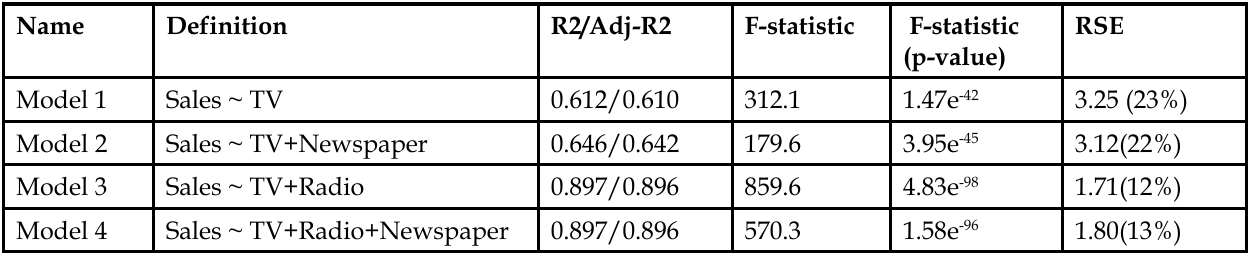
\includegraphics[width=10cm,keepaspectratio=true]{./images/modelsGuide.png}
	% modelsGuide.png: 0x0 pixel, 300dpi, 0.00x0.00 cm, bb=
	\caption{Guía para la selección de variables.}
	\label{fig:modelsGuide}
\end{figure}


[]{}
Finalmente, para resumir, para un buen modelo lineal, los predictores deberían escogerse con base en los siguientes criterios:
\begin{itemize}
	\item \texttt{$R^2$}: Este valor siempre aumentará cuando se agregue una nueva variable de predicción al
	modelo. Sin embargo, no es una verificación muy confiable de la mayor eficiencia de
	el modelo. Más bien, para un modelo eficiente, debemos verificar el $R^2$ ajustado.
	Esto debería aumentar al agregar una nueva variable de predicción.
	\item \texttt{valor$-p$}: Cuanto menor sea el valor$-p$ para la estimación de la variable de predicción,
	mejor es agregar la variable de predicción al modelo.
	\item \texttt{Estadístico$-F$}: El valor del estadístico$-F$ para el modelo debería aumentar después de
	la adición de una nueva variable de predicción para considerarse una
	adición eficiente al modelo. El aumento en el estadístico$-F$ es un buen indicador para la mejora en el modelo debida únicamente por la adición de ese variable particular. Alternativamente, el valor$-p$ asociado con el estadístico $F$ debería disminuir al agregar una nueva variable de predicción. 
	\item \texttt{RSE}: Este valor para el nuevo modelo debería disminuir al agregar
	la nueva variable de predicción.
	\item \texttt{VIF}: Para ocuparse de los Problemas que surgen debido a la colinealidad múltiple, se necesita
	eliminar las variables con grandes valores \texttt{VIF}.
\end{itemize}

